\section{Water Orientation}

Previous studies have provided a detailed overview of water orientation at the interface with both air and organic phases.\cite{McFearin2009,Hore2008,Fan2009,Wick2006c,Wick2008a} The topmost water layers are highly disrupted because of their contact with the organic phase, and it has been suggested that ordering of both the organic and water molecules would lead to a field across the boundary of the interface.\cite{McFearin2009,Hore2008} This can influence charged species, and the ordering and orientation of the H-bond network. Our recent experimental SFG results suggest that the accumulation of charged ions leads to a field-screening that affects the orientation of waters in the topmost layers. This is complemented by the results of the current study.

\begin{figure}[h!]
\begin{center}
	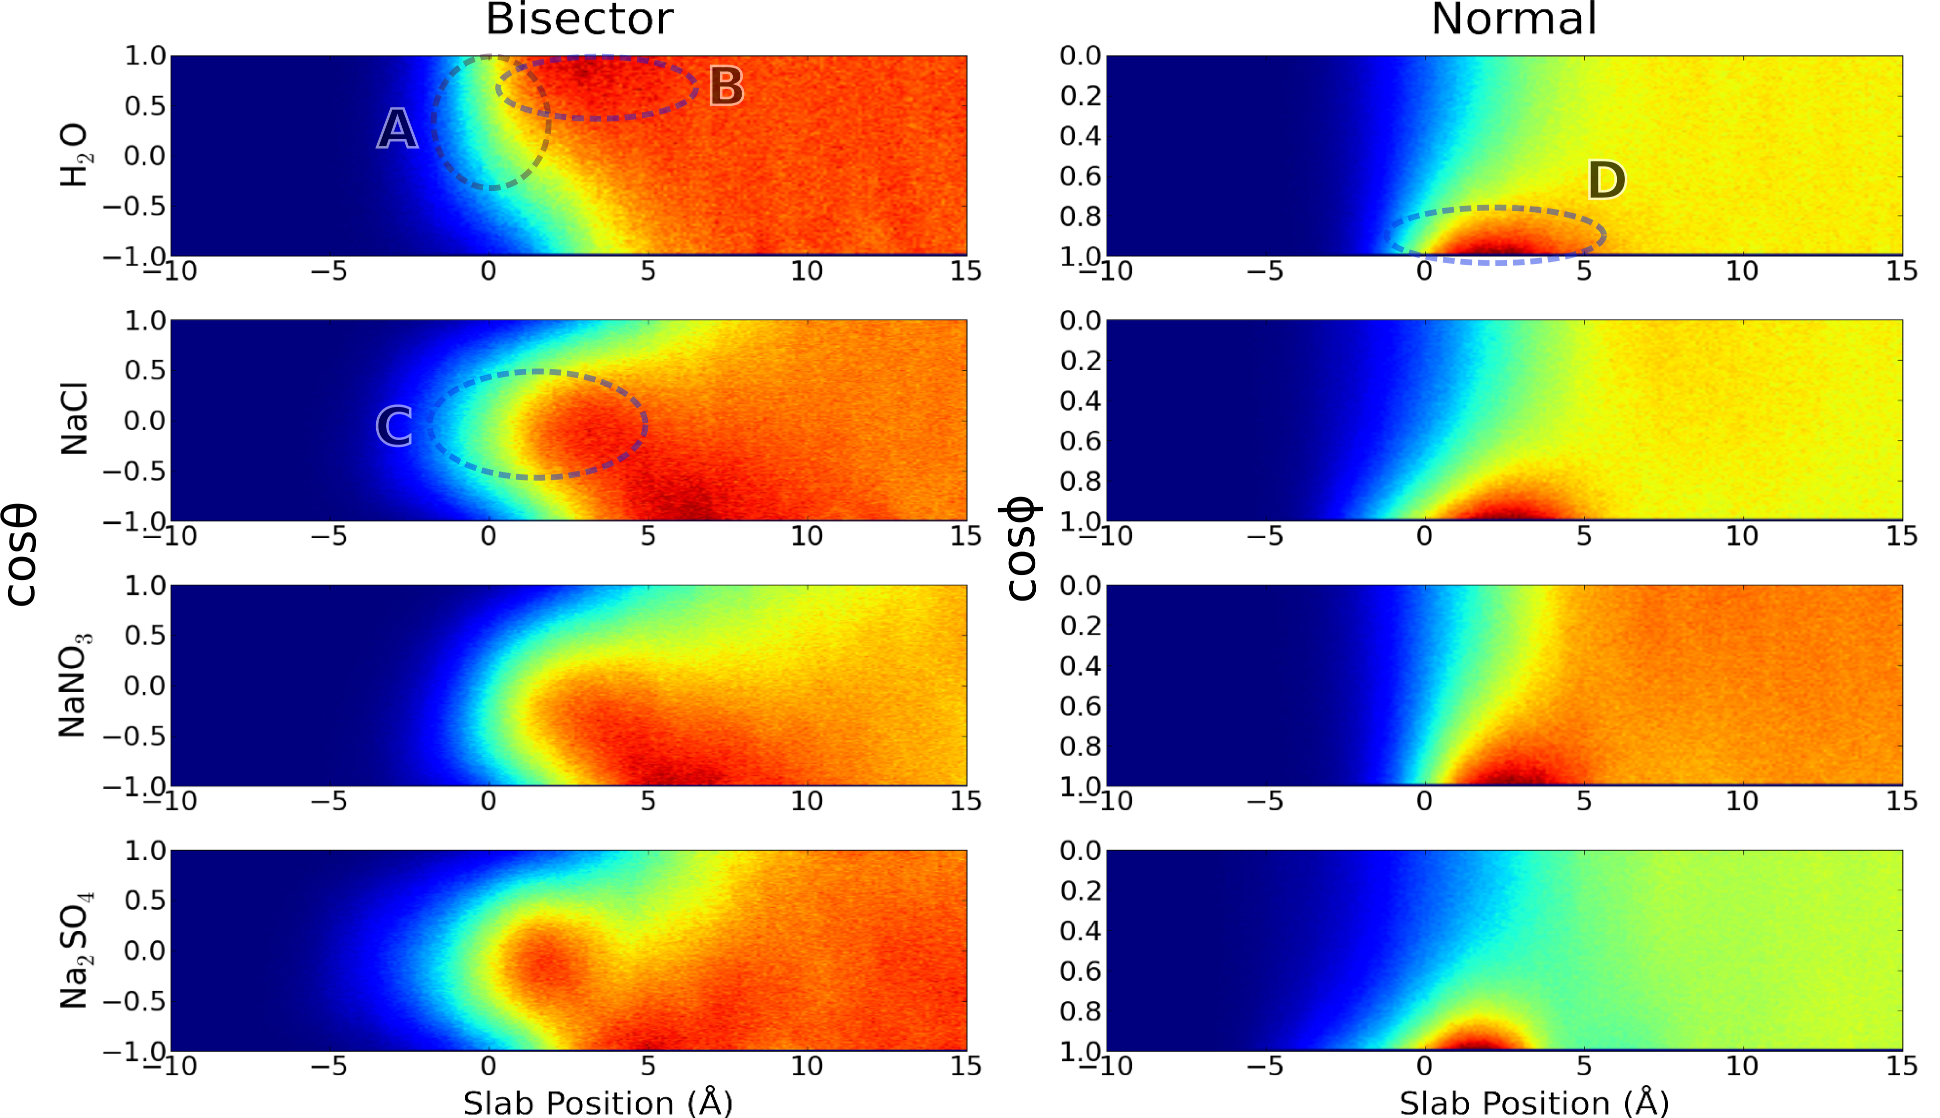
\includegraphics[scale=1.0]{images/h2o-2dhistograms.png}
	\caption{Orientation profiles of interfacial water molecules at different depths from the GDS. The molecular bisector profile (left column) and the profile of the molecular axis normal to the plane of the water molecule (right column) are shown. Both angle definitions are depicted in Figure \ref{fig:water-angles}, and the angle cosines are plotted here. The neat-\ctcwat, \nacl, \sodnit, and \sodsul~system water orientation profiles are plotted from top to bottom row, respectively. Positive position values indicate the aqueous phase, and negative positions are in the \ctc~phase. Regions labeled in the profile correspond to orientations depicted in Figure \ref{fig:angle-ranges}.}
	\label{fig:2dhisto}
\end{center}
\end{figure}


The orientation of water within the aqueous/organic interface of the system was defined using the angles formed by molecular axes and the fixed reference axis of the system (perpendicular to the interfacial plane), as described previously, and as depicted in Figure \ref{fig:water-angles}. Figure \ref{fig:2dhisto} shows the angle profiles of both the molecular bisector and the molecular plane normal of water molecules relative to the system reference axis at various depths into the aqueous phase. Darker red regions of the plots indicate higher orientational populations, while homogeneous coloring across the angle range indicates orientational isotropy.

\newcommand{\degree}{\ensuremath{^\circ}}

\begin{figure}[h!]
\begin{center}
	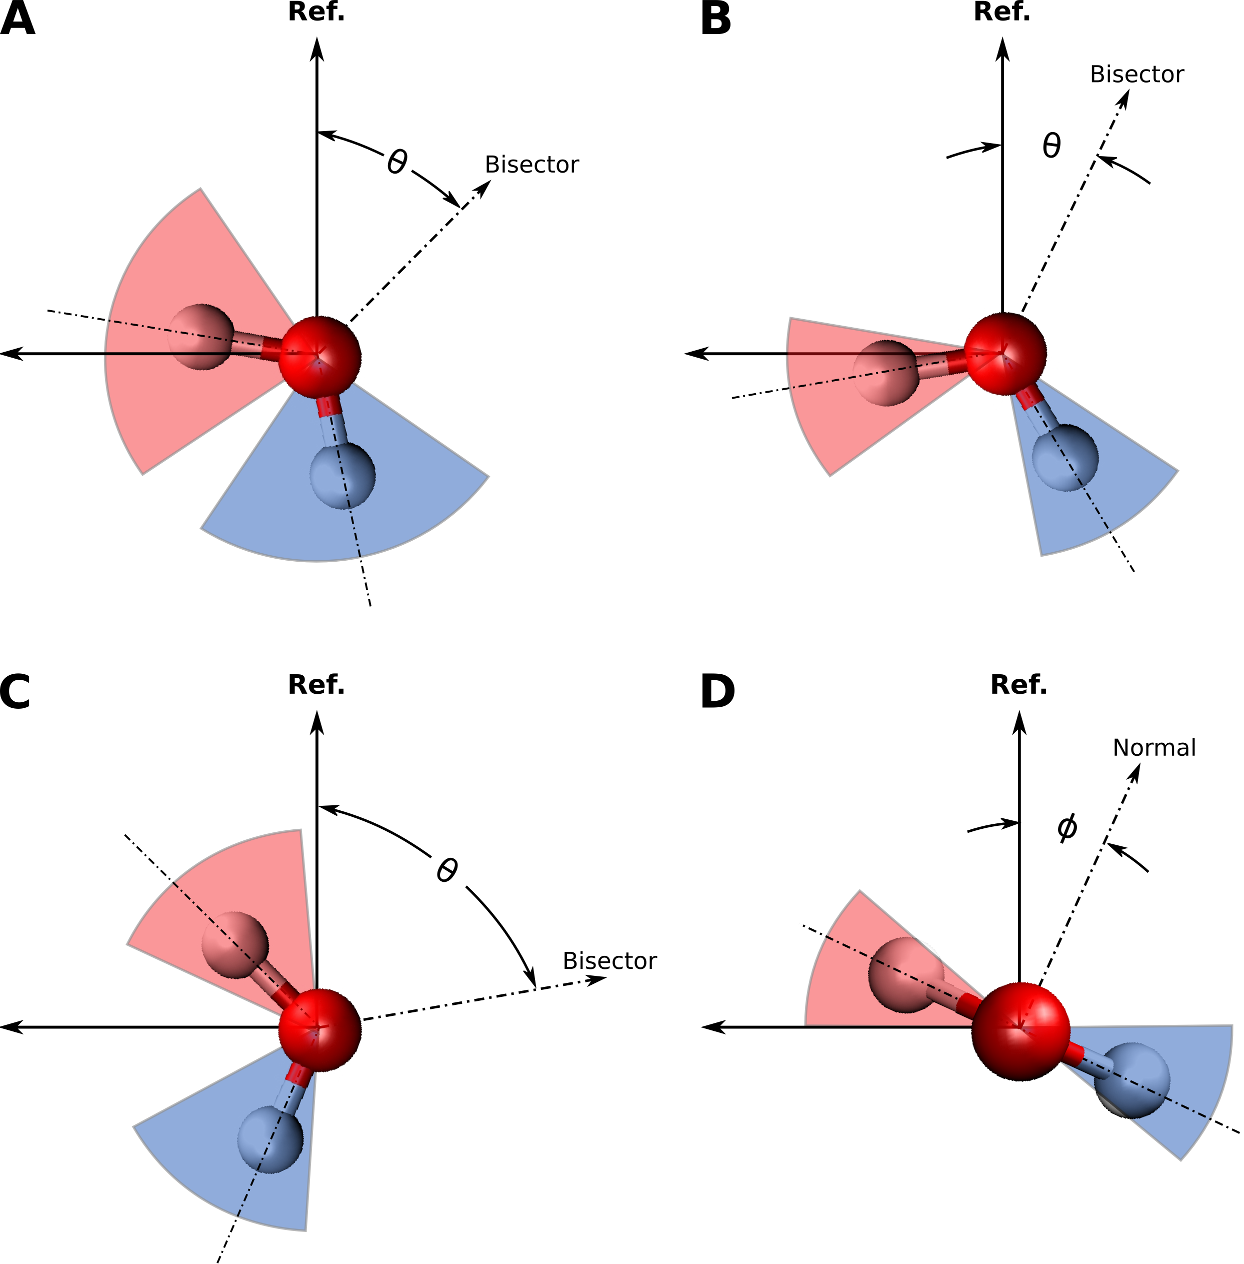
\includegraphics[scale=1.0]{images/h2o-angle-ranges.png}
	\caption{Depictions of water orientations ranges spanning varying values of $\theta$ and $\phi$, as defined in Figure \ref{fig:water-angles}. The effect of rotating the water within a fixed angle range is illustrated by the shaded (red and blue) regions that bound the OH-bonds. Ranges of $\theta$ shown here are (A) 0\costhetarange1, (B) 0.7\costhetarange1, (C) -0.5\costhetarange0.5. (D) The $\phi$ range of 0.7\cosphirange1 shows the molecular plane of the water mostly flat (i.e. parallel to) the plane perpendicular to the reference axis. Depictions here correspond to those regions labeled in Figure \ref{fig:2dhisto}.}
	\label{fig:angle-ranges}
\end{center}
\end{figure}

In the left column of Figure \ref{fig:2dhisto} are the bisector orientation profiles for each of the systems. The far-left dark-blue regions of the plots show the \ctc~bulk near the interface where few or no waters are found. The GDS is located at a depth of 0.0\ang. To the far right in the water bulk, the flat, uniformly-colored profile represents the expected isotropic orientation of the bulk waters. The regions of interest lie around the GDS within the interface. The top bisector profile is that of the neat-\ctcwat~system, and it shows a transition in the profile beginning approx. 2\ang~into the \ctc~phase, and extending up to 5\ang~into the aqueous side, at which point the profile becomes orientationally isotropic. At the GDS most of the waters are oriented between 0.0\costhetarange1.0, indicating a range of orientations as depicted in Figure \ref{fig:angle-ranges}a. In this range one of the OH-bonds points into the aqueous side, and the other straddles the interfacial plane with a slight affinity towards the organic \ctc~phase. Just under the water surface, between 2-4\ang~into the neat-\wat phase, a dark-red region spanning approx. 0.7\costhetarange1.0 appears. This narrow orientational range is depicted in Figure \ref{fig:angle-ranges}b, and is similar to the waters in the topmost aqueous layer nearer to the GDS, but further limited such that one OH bond points into the \wat side, and one straddles the interfacial plane with a tendency to point into the \wat phase.

The reference \ctcwat~bisector orientational profile is comparable to previous simulations of the same system. Using slightly different simulation parameters for the same reference \ctcwat~system, Wick and Dang found the free-OH to point slightly into the \ctc~phase at the GDS with an angle of \costheta$_{free-OH}\approx 0.4$.\cite{Wick2006c} This corresponds to \costheta$_{bisector} \approx 0.5$ in the this work's angle definition. Similarly, deeper into the surface the angle profile diminishes such that $\cos(\theta_{free-OH})\approx 0.0$ within 5\ang~of the GDS, corresponding to $\cos(\theta_{bisector})\approx 0.8$ in the current scheme. Those results agree with this work's reference \ctcwat~profile, further complementing the experimental conclusions performed on the same systems.\cite{McFearin2009,Scatena2001}

Bisector angle profiles for the salt systems show different behavior than that of the reference neat \ctcwat~system. The profiles of the salt systems at the GDS all center about the \costheta$=0$ region, with a range of approx. -0.5\costhetarange0.5. This indicates a straddling water molecule with the orientational range depicted in Figure \ref{fig:angle-ranges}c. The water in that range is clearly oriented such that one OH-bond always points out of the aqueous phase into the \ctc, and the other always points in to the water bulk. The OH-bond that would straddle the interface in the reference system points out of the interface with a greater angle. This orientation, centered about \costheta$\approx 0$, extends into the water phase up to 3\ang, at which point the profile shifts to the darker region near -1.0\costhetarange0.7. The sub-surface region of the profile between 4-7\ang~in each system corresponds to a flip of the water orientation, as referred to in a recent SFG study as a ``flip-flop'' model where water orients to counteract the field of charged species at interfaces.\cite{Nihonyanagi2009} The cation density enhancement in each salt system is within the region approx. 5-7\ang~below the GDS. The waters may be orienting with the negatively charged oxygen end towards those cations, and with the field established by the ion double-layer within the interface. In each of the salt bisector profiles there is a clear depletion of waters oriented towards \costheta$=1$ suggesting that alignment of the bisector with the reference axis is not preferred. The effect is most pronounced in the \sodsul~system where the distance between counter-ion density enhancements is smallest, and the transition in the bisector profile is the most abrupt, changing from a profile mostly in the range of -1.0\costhetarange0.5 to isotropic orientation quickly near 8\ang~into the aqueous phase. The \sodnit~system bisector profile shows the effect furthest into the water bulk, extending almost to 13\ang. Counter-ion density enhancement is most separated in \sodnit, however, and most of the orientational affinity for -1.0\costhetarange0.5 occurs within the first 10\ang~of the surface. The bisector profile of the \nacl~system is broadest with -1.0\costhetarange0.7 starting near the GDS. Also, orientational isotropy is shallowest in the \nacl~system starting near 7\ang~into the aqueous phase.

It appears that the field established by the anion-cation pairing within the interface affects the depth to which waters are oriented before the bulk isotropic profile begins. Also, the range of orientations beneath the surface is dependent on the properties of the anion. The weakly polarizable \cl~anion does not restrict the orientational range as much as the more polarizable \nit~and \sul. Anions also appear to control the depth to which the water orientation is felt, with the most surface-active \nit~anion causing the deepest effect. \sul~anion shows the strongest restriction on the range of bisector angles, and the sharpest orientational transition to the bulk, which may be attributed to the higher charge of the anion, and thus the stronger field established between the counter-ions in the system.

\newcommand{\phiprof}{$\phi$-profile~}

Orientational profiles for the molecular plane normal of the water molecules ($\phi$-profiles) are found in the right-column of Figure \ref{fig:2dhisto}. The range of a \phiprof is limited to 0.0\cosphirange1.0 because of the inherent symmetry of the plane of the water molecule. More similarity is shared between the $\phi$-profiles than the bisector profiles for the different systems. The neat \ctcwat~$\phi$-profile is typical of the other systems in appearance, with a large clustering of water population in the range of 0.7\cosphirange1.0 between the GDS and up to 7\ang~into the aqueous phase. This particular $\phi$ range is depicted in Figure \ref{fig:angle-ranges}d, showing the mostly flat (i.e. parallel to the interface) orientation of the molecular plane. It is notable that the $\phi$-orientation is affected to the same depth as the first peak (dark-red region) of the bisector profile. However, in the salt systems the second peak near to \costheta$=-1.0$ begins at a depth where the \phiprof has already become isotropic. Thus, in the salt systems, the first water layer (between the GDS and almost 4\ang~into the surface) has a defined $\phi$-orientation that is rather flat on the interfacial plane, but the deeper waters (4-7\ang~into the interface) are isotropic in $\phi$, and oriented with \costheta closer to -1.0 (an orientation with oxygen pointing into the water bulk, and hydrogens more towards the interface).

By virtue of the interdependence of $\theta$ and $\phi$ (the bisector is perpendicular to the molecular plane normal at all times) a value of \cosphi$=1.0$ implies \costheta$=0$, and vice-versa. However, a broad $\theta$-range allows for a full range of $\phi$ values. Although the second peak of the salt-system bisector profiles is concentrated near to \costheta$=-1.0$, the corresponding \phiprof is isotropic. This deeper region (the second water layer) orients with the bisector counteracting the field of the anion-cation double-layer, and the only apparent affinity is that of placing oxygen closer to the cation density enhancement (and hydrogen closer to the anion layer), while the \phiprof spans the entire orientational range.

